
\section{Preparazione e misure magnetiche per complessi di \ce{Ni(II)}}

\subsection{Preparazione di \ce{Ni(en)3Cl2.2H2O} }
\begin{figure}[ht!]
    \centering
    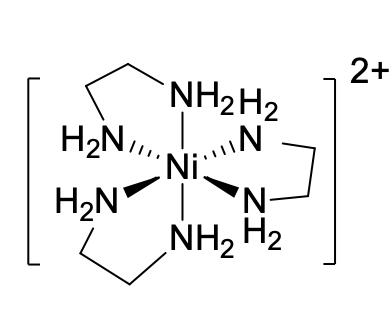
\includegraphics[width=0.3\linewidth]{foto/nien.png}
    \caption{Complesso \ce{Ni(en)3Cl2} }
    \label{fig:nien}
\end{figure}
\subsubsection{Procedura sperimentale}
Abbiamo pesato alla bilancia tecnica $3.00 \mathrm{~g}$ di $\mathrm{NiCl}_2 \cdot 6 \mathrm{H}_2 \mathrm{O}$\footnote{ E' stato utilizzato il nichel cloruro anidro, la massa pesata quindi differisce dal valore prestabilito dalle dispense. Nella sezione dedicata ai calcoli si utilizza la massa aggiustata per il sale anidro} e li abbiamo disciolti in un becher con $1.5 \mathrm{~mL}$ d'acqua sotto agitazione e con l'aiuto di un debole riscaldamento. Nello stesso recipiente abbiamo aggiunto $2.8 \mathrm{~mL}$ di etilendiammina e immerso il tutto in un bagno di ghiaccio. Si osserva la precipitazione di un complesso viola. In seguito abbiamo addizionato tramite cilindro graduato $7.5 \mathrm{~mL}$ di etanolo freddo come non solvente per favorire la cristallizzazione. Quindi abbiamo filtrato su Buchner e lavato con due aliquote da $5.0 \mathrm{~mL}$ di etanolo. Infine, dopo aver asciugato sul Buchner i cristalli, li abbiamo trasferiti in una provetta precedentemente pesata alla bilancia analitica per essere seccati sottovuoto alla pompa meccanica.
\subsubsection{Commenti e osservazioni}
La dissoluzione del solido è stata difficoltosa, abbiamo dovuto scaldare e far scorrere l'ancoretta su tutto il fondo del becher per diversi minuti. Questo può essere dovuto alla granulometria del nichel che si era "cementificato" formando degli agglomerati duri difficili da rompere tramite agitazione magnetica. Alcune possibili soluzioni a questo problema possono essere: evitare questi granuli durante la pesata, pestellare il solido per omogenizzare il solido( questo può essere eseguito nel becher con una bacchetta di vetro oppure in un mortaio, in quest'ultimo caso l'operazione va eseguita prima della pesata in quanto altrimenti avremo che parte del solido rimarrebbe attaccata alle pareti del pestello e del mortaio).
Abbiamo notato inoltre la variazione di colore non è stata diretta ma è passata per colorazioni intermedie. Questo fenomeno può essere spiegato dal fatto che la completa complessazione procede per specie intermedie come \ce{[Ni(en)(OH2)4]^{2+} }, \ce{[Ni(en)2(OH2)2]^{2+} } \footnote{Si presume che ulteriori intermedi come \ce{[Ni(en)(OH2)5]^{2+} } e  \ce{[Ni(en)2(OH2)3]^{2+} } si convertano abbastanza velocemente da provocare transizioni di colore visibili della soluzione  }


\subsubsection{Calcoli e analisi dei dati}

Il numero di moli di $\mathrm{NiCl}_2 \cdot 6 \mathrm{H}_2 \mathrm{O}$ che occorrono sono
$$
n_{\mathrm{NiCl}_2}=\frac{3.00 \mathrm{~g}}{237.70 \mathrm{~g} / \mathrm{mol}}=0.0126 \mathrm{~mol}
$$
che convertite in massa di \ce{NiCl2} anidro da pesare si trasformano in

\[  {m_{\ce{NiCl2}}} = n_{\mathrm{NiCl}_2} \cdot {M_{\ce{NiCl2}}} = 0.0126 \mathrm{~mol} \cdot 129.6  \ \text{g/mol} = 1.63 \text{g} \]
Per l'etilendiammina
$$
n_{\mathrm{en}}=\frac{2.8 \mathrm{~mL} \cdot 0.899 \mathrm{~g} / \mathrm{mL}}{237.7 \mathrm{~g} / \mathrm{mol}}=0.0419 \mathrm{~mol}
$$
Notiamo che l'etilendiammina è in eccesso, infatti il rapporto $\frac{n_{\text{en}}}{{n_{\ce{NiCl2}}}} = 3.33 > 3$
Di conseguenza, poiché l'etilendiammina è più che stechiometrica, deduciamo che il reagente limitante è il sale di nichel. 

La resa sarà dunque calcolata basandosi sul nichel iniziale\footnote{Un eccesso di etilendiammina è necessario per garantire la completa complessazione del nichel a tris(etilendiammina)nichel dicloruro. Questo non inficerà la purezza del prodotto in quanto l'eccesso sarà rimossa dai lavaggi con etanolo}. 
La massa di prodotto ottenuta ottiene facendo la differenza fra la massa della provetta piena dopo l'essiccazione sottovuoto e quella della provetta vuota:
$$
m_{\text {prod }}=21.4424  \mathrm{~g}- 15.1714 \mathrm{~g}= 4.2710 \mathrm{~g}
$$
Il numero di moli di prodotto è quindi
$$
n_{\text {prod }}=\frac{4.2710 \mathrm{~g}}{345.92 \mathrm{~g} / \mathrm{mol}}=0.0112 \mathrm{~mol}$$ 

$$Y_\% = \frac{n_\text{prod}}{n_{\mathrm{NiCl}_2}}\cdot 100 = \frac{0.01235 \mathrm{~mol}}{0.0126 \mathrm{~mol}} \cdot 100 =98 \%
$$
La resa della reazione concorda con quella presente in letteratura \cite{support}
\subsection{Preparazione di \ce{[Ni(Et2en)2(H2O)2]Br2 } e \ce{[Ni(Et2en)2Br2]}}
\begin{figure}[ht!]
    \centering
    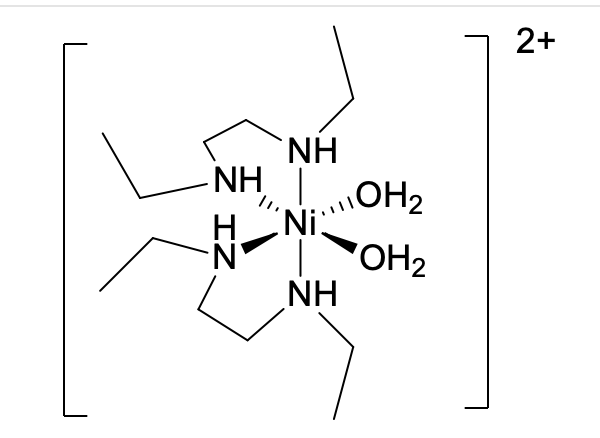
\includegraphics[width=0.4\linewidth]{foto/nieten2.png}
    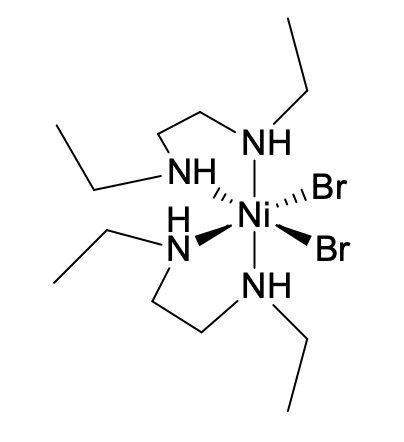
\includegraphics[width=0.265\linewidth]{foto/nietenbr2.png}
    \caption{A sinistra troviamo \ce{[Ni(Et2en)2(H2O)2]Br2 } mentre a destra \ce{[Ni(Et2en)2Br2]} }
    \label{fig:nieten}
\end{figure}



\subsubsection{Procedura sperimentale}

Abbiamo preparato una soluzione di bromuro di nichel sciogliendo $1.36 \mathrm{~g}$ di $\mathrm{NiBr}_2 \cdot 3 \mathrm{H}_2 \mathrm{O}$ in $30 \mathrm{~mL}$ di etanolo. Successivamente abbiamo aggiunto  $1.4 \mathrm{~mL}$ di $\mathrm{Et}_2 \mathrm{en}$\footnote{ Quantità corrispondente a 1.6 g prescritti nelle dispense}. Precipita un solido di colore verde acqua che dopo qualche ora dovrà essere filtrato su Buchner e lavato con etanolo. Lasciato seccare sul filtro sotto all'azione della pompa, si trasferisce in una provetta precedentemente pesata per poi essiccarlo sottovuoto. Dopo aver pesato la provetta contenente il sale ormai asciutto trasferisco, successivamente ne metà del suo contenuto in un'altra provetta precedentemente pesata che colloco in stufa per rimuovere l'acqua dalla sfera di coordinazione interna. Infine, il giorno successivo si pesa la provetta e si calcola la perdita d'acqua.

\subsubsection{Commenti e osservazioni}
Una scarsa dimestichezza con le operazioni di filtrazione ci ha fatto terminare precocemente la filtrazione lasciando il solido sul filtro ancora bagnato\footnote{In parte è anche colpa della particelle del solido, che essendo molto piccole hanno trattenuto molta acqua e creato una pasta molto densa e corposa che ha rallentato l'essiccamento sul filtro}.
Questo ha provocato la formazione di una pasta molto densa è appiccicosa che è rimasta su tutta l'attrezzatura riducendo la quantità di prodotto finale ottenuto.
Abbiamo notato un cambio colorazione successivo al trattamento del prodotto idrato in stufa. Una volta finito il processo di essiccamento si potevano distinguere le due porzioni; quella trattata e quella no.
\subsubsection{Calcoli e analisi dati}

Il numero di moli di \ce{NiBr2.3H2O} che occorrono sono
$$
n_{\mathrm{NiBr}_2}=\frac{1.36 \mathrm{~g}}{272.55 \mathrm{~g} / \mathrm{mol}}=4.990 \mathrm{~mmol}
$$
Sulle dispense erano riportata la massa da prelevare, avendo a disposizione una pipetta dobbiamo convertire il dato in un volume

\[ V = \frac{m}{\rho} = \frac{1.16\um{g}}{0.827 \um{g/mL}} = 1.4 \um{mL} \]


per \ce{Et2en} $\rho = 0.827 \um{g/mL}$
$$
n_{\mathrm{Et}_2 \mathrm{en}}=\frac{1.4 \mathrm{~mL} \cdot 0.827 \mathrm{~g} / \mathrm{mL}}{116.20 \mathrm{~g} / \mathrm{mol}}=9.96 \mathrm{~mmol}
$$
Poiché la stechiometria del prodotto è $1: 2$ si ricava che il reagente limitante è la N,N-dietiletilendiammina. 

Calcoliamo la resa 
\[ Y_\% = \frac{n_\text{pro}}{n_{\mathrm{NiBr}_2}}\cdot 100 \]

Le moli finali sono il rapporto massa della provettà piena di prodotto tolta la tara e la massa molare del prodotto.

\[ n_\text{pro} = \frac{m_{f} - m_{t}}{M_\text{pro}} 
 = \frac{ 17.1101\um{g} - 15.0134 \um{g}}{ 486.93 \um{g/mol}} =  \frac{2.097 \mathrm{~g}}{486.93 \mathrm{~g} / \mathrm{mol}}=4.306 \um{mmol}\]

\[ Y_\% = \frac{n_\text{pro}}{n_{\mathrm{NiCl}_2}}\cdot 100  = \frac{2 \cdot 4.306 \cdot 10^{-3} \mathrm{~mol}}{9.96 \cdot 10^{-3} \mathrm{~mol}} \cdot 100 =86.5 \%\]


Calcoliamo ora la perdita di peso della frazione lasciata in stufa. Abbiamo pesato $ 0.8751  \um{g} $ di composto e ci siamo segnati la tara   $ 20.7369\um{g}$. Dopo la disidratazione la massa della provetta era $ 21.6770 \um{g}$. La perdita netta di peso teorica è: 

\[ \Delta m =\frac{ 2\cdot M_{\ce{H2O}}}{M_{\text{pro}} } m_{\text{pesata}} \]

Vediamo che il $\Delta m$ sperimentale è 
\[ \Delta m = m_f -(m_{\text{tara}} +m_{\text{pro}}) = 21.6770 \um{g} - 20.7369 \um{g} - 0.8751   \um{g} = 0.065\um{g}\]
\subsection{Preparazione di {\ce{[Ni(NH3)6] }}}

\begin{figure}[ht!]
    \centering
    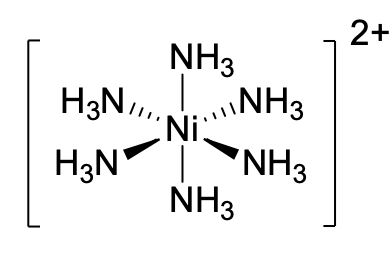
\includegraphics[width=0.3\linewidth]{foto/ninh3.png}
    \caption{Complesso \ce{[Ni(NH3)6] }}
    \label{fig:ninh3}
\end{figure}
\subsubsection{Procedura sperimentale}
Abbiamo preparato una soluzione di cloruro di nichel sciogliendo di $3.00$ g \ce{NiCl2} $\cdot$ 6\ce{H2O} 
in 5 mL di \ce{H2O} a caldo. Successivamente abbiamo aggiunto $5.8$ mL di \ce{NH4OH} concentrato. Si raffredda usando un bagno di ghiaccio si completa la precipitazione aggiungendo etanolo. Si filtra il precipitato su Buchner, si trasferisce in una provetta precedentemente pesata e si asciuga sotto vuoto. Si pesa il prodotto asciutto e si calcola la resa di reazione
\subsubsection{Commenti e osservazioni}
La reazione è avvenuta senza imprevisti. Dopo l'aggiunta dell'idrossido di ammonio si è subito notata la variazione di colore. Come si vede dai calcoli, si utilizza un largo eccesso di idrossido di ammonio in quanto la reazione di complessazione è un equilibrio, aggiungendo un reagente l'equilibro verrà spostato verso la formazione dei prodotti. Il successivo raffreddamento e l'aggiunta di etanolo incentiveranno la formazione di prodotto e sarà rimosso dall'ambiente di reazione favorendo la complessazione. Il complesso è idrolabile se lasciato in acqua pura l'ammoniaca viene liberata e si riforma l'esaacquo-ione di partenza. Come per il complesso precedente abbiamo utilizzato il cloruro anidro quindi la massa effettiva di solido pesata era minore.




\subsubsection{Calcoli e analisi dei dati}
Come prima, il numero di moli di $\mathrm{NiCl}_2 \cdot 6 \mathrm{H}_2 \mathrm{O}$ che occorrono sono
$$
n_{\mathrm{NiCl}_2}=\frac{3.00 \mathrm{~g}}{237.70 \mathrm{~g} / \mathrm{mol}}=0.0126 \mathrm{~mol}
$$
che convertite in massa di \ce{NiCl2} anidro da pesare si trasformano in

\[  {m_{\ce{NiCl2}}} = n_{\mathrm{NiCl}_2} \cdot {M_{\ce{NiCl2}}} = 12.6 \text{mmol} \cdot 129.6  \ \text{g/mol} = 1.63 \text{g} \]

Calcoliamo le moli di ammoniaca aggiunte, sappiamo che una soluzione concentrata di idrossido di ammonio è circa $18$ M \cite{ammonia}, quindi in $5.8$ mL ci sono

\[ n_{\ce{NH3}} = C \cdot V = 18\um{mmol/mL} \cdot 5.8 \ \text{mL} = 104.4 \um{mmol} \]

Ora calcoliamo la resa sulle moli di nichel iniziali
\[ Y_\% = \frac{n_\text{pro}}{n_{\mathrm{NiCl}_2}}\cdot 100 \]

Le moli finali sono il rapporto massa della provettà piena di prodotto tolta la tara e la massa molare del prodotto.

\[ n_\text{pro} = \frac{m_{f} - m_{t}}{M_\text{pro}} 
 = \frac{17.7280 \um{g} - 15.1515\um{g} }{ 231.78 \um{g/mol}} = 0.01112 \um{mol}\]

\[ Y_\% = \frac{n_\text{pro}}{n_{\mathrm{NiCl}_2}}\cdot 100  = \frac{0.01112 \um{mol}}{0.0126 \um{mol}} \cdot 100 = 88.2\% \]
La resa concorda con quanto viene riportato in letteratura \cite{support}
\subsection{Caratterizzazione UV-VIS}
\subsubsection{Procedura sperimentale}
Si preparano 3 soluzioni circa 0.1 M dei tre sali portando a volume con acqua \ce{[Ni(en)3]Cl2.2H2O} e \ce{[Ni(Eten)2H2O]Br2}
mentre con \ce{NH4OH} 3 M \ce{[Ni(NH3)6]Cl2}\footnote{Come già detto \ce{[Ni(NH3)6]Cl2} si  idrolizza se sciolto in acqua.}
La polvere da pesare per ottenere una soluzione di quella concentrazione in un matraccio da 50 mL\footnote{Abbiamo fatto questa scelta di volume per non dover utilizzare troppo campione ma comunque mantenendo una quantità tale mantenere precisa la pesata. Per il \ce{[Ni(Eten)2H2O]Br2} abbiamo scelto un matraccio da 10 mL perché non avevamo abbastanza prodotto per fare l'analisi.}

\[ m_{\ce{[Ni(NH3)6]Cl2}} = C \cdot V_{\text{matraccio}} \cdot M_{\ce{[Ni(NH3)6]Cl2}}  = 0.1 \um{M} \cdot 50 \um{mL} \cdot 231.78 \um{g/mol} = 1.1589 \um{g} \]

\[ m_{\ce{[Ni(en)3]Cl2}} = C \cdot V_{\text{matraccio}} \cdot M_{\ce{[Ni(en)3]Cl2.2H2O}}  = 0.1 \um{M} \cdot 50 \um{mL} \cdot 345.92 \um{g/mol} = 1.7296 \um{g} \]

\[ m_{\ce{[Ni(en)3]Cl2}} = C \cdot V_{\text{matraccio}} \cdot M_{\ce{[Ni(en)3]Cl2.2H2O}}  = 0.1 \um{M} \cdot 10 \um{mL} \cdot 486.93 \um{g/mol} = 0.4689\um{g} \]

In  \autoref{tab:pesate} sono presenti i valori pesati dei tre sali.
\subsubsection{Spettri}


\begin{figure}[ht!]
    \centering
    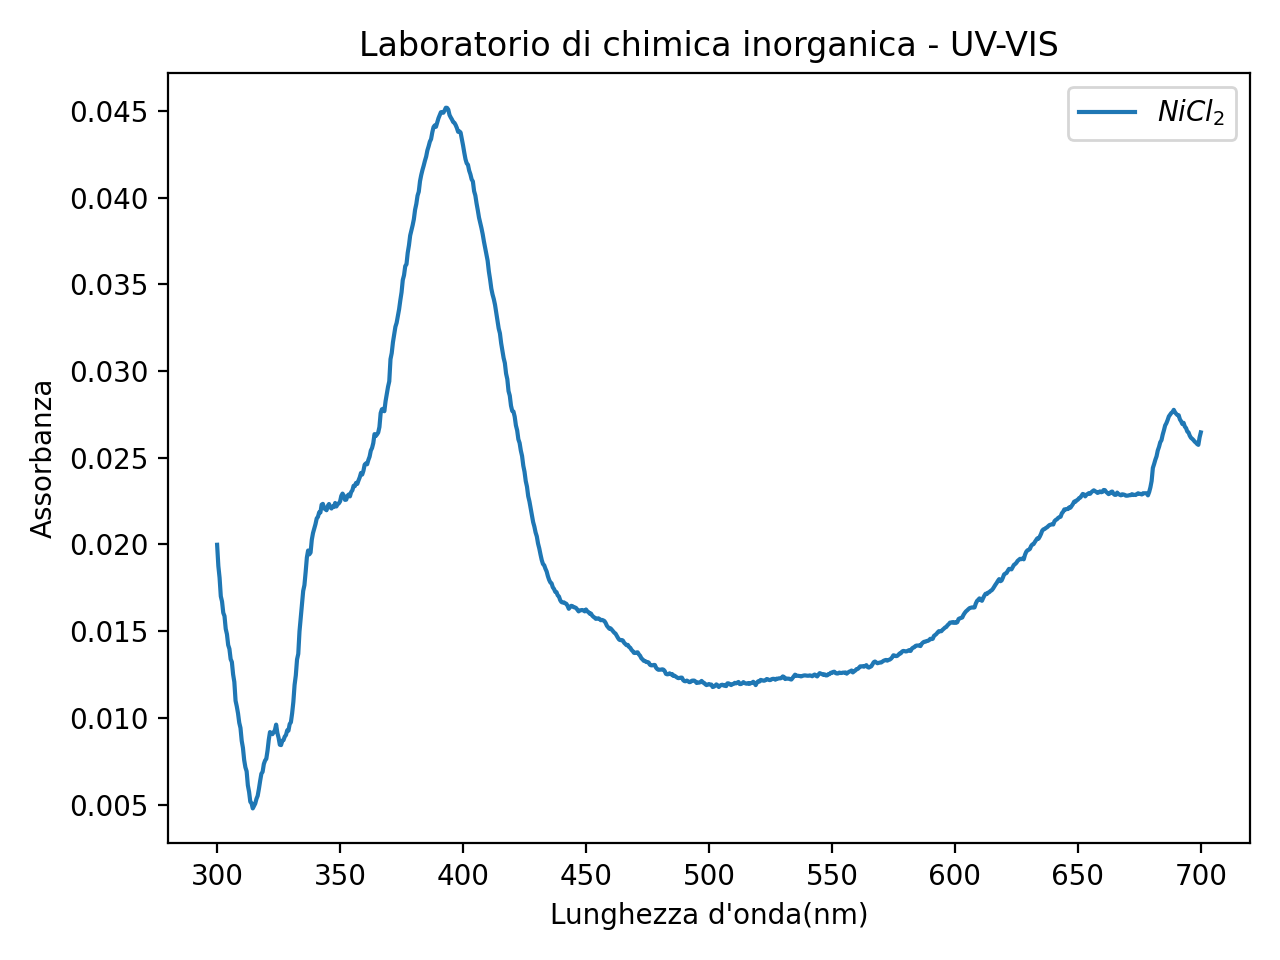
\includegraphics{Relazione/foto/nicl2uv.png}
    
    \caption{Spettro UV-VIS \ce{NiCl2}}
    \label{fig:nicl2uv}
\end{figure}

\begin{figure}[ht!]
    \centering
    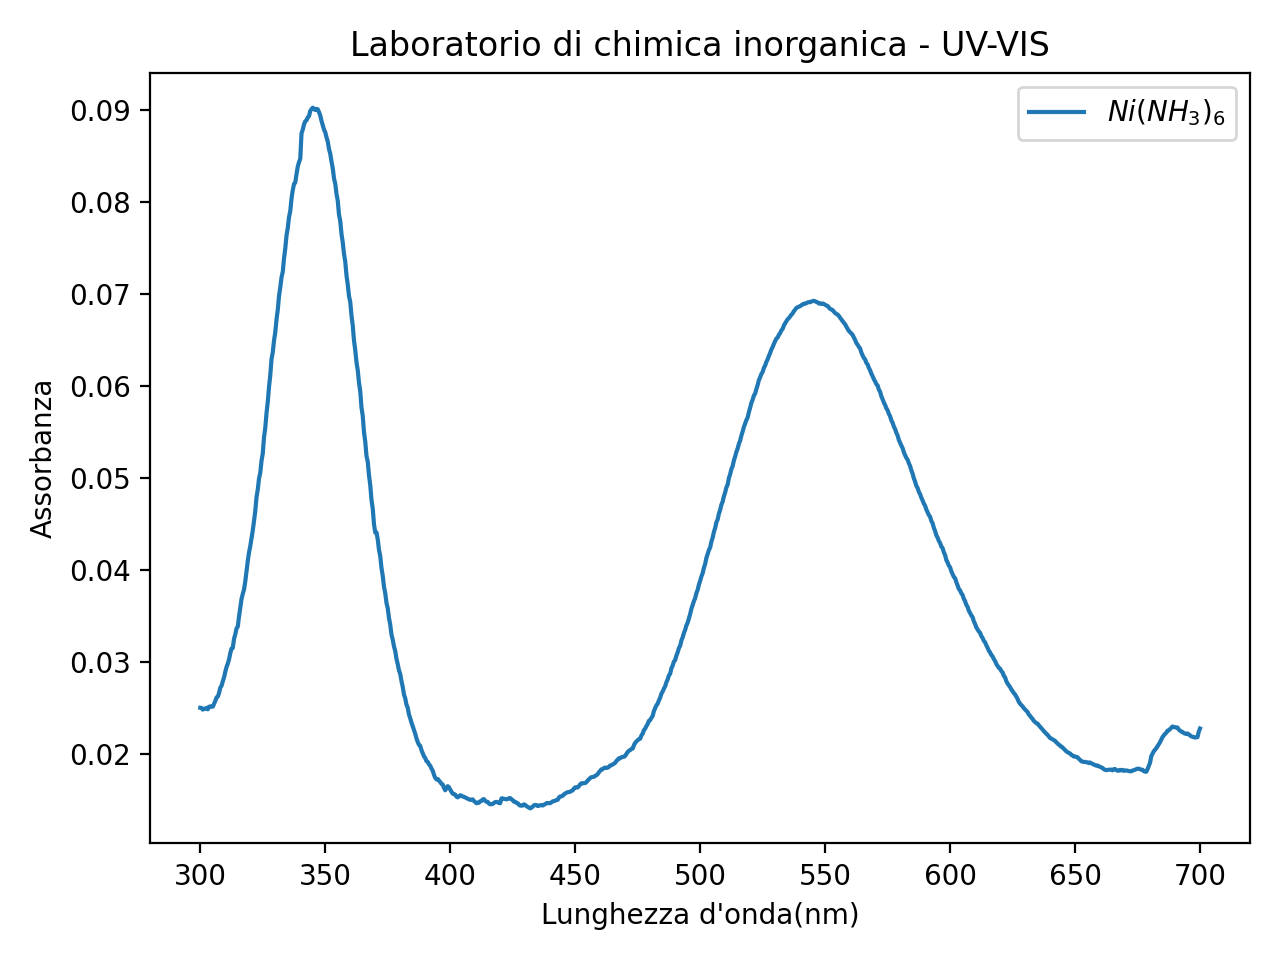
\includegraphics{Relazione/foto/ninh3uv.png}
    
    \caption{Spettro UV-VIS \ce{[Ni(NH3)6]Cl2}}
    \label{fig:ninh3uv}
\end{figure}
\begin{figure}[ht!]
    \centering
   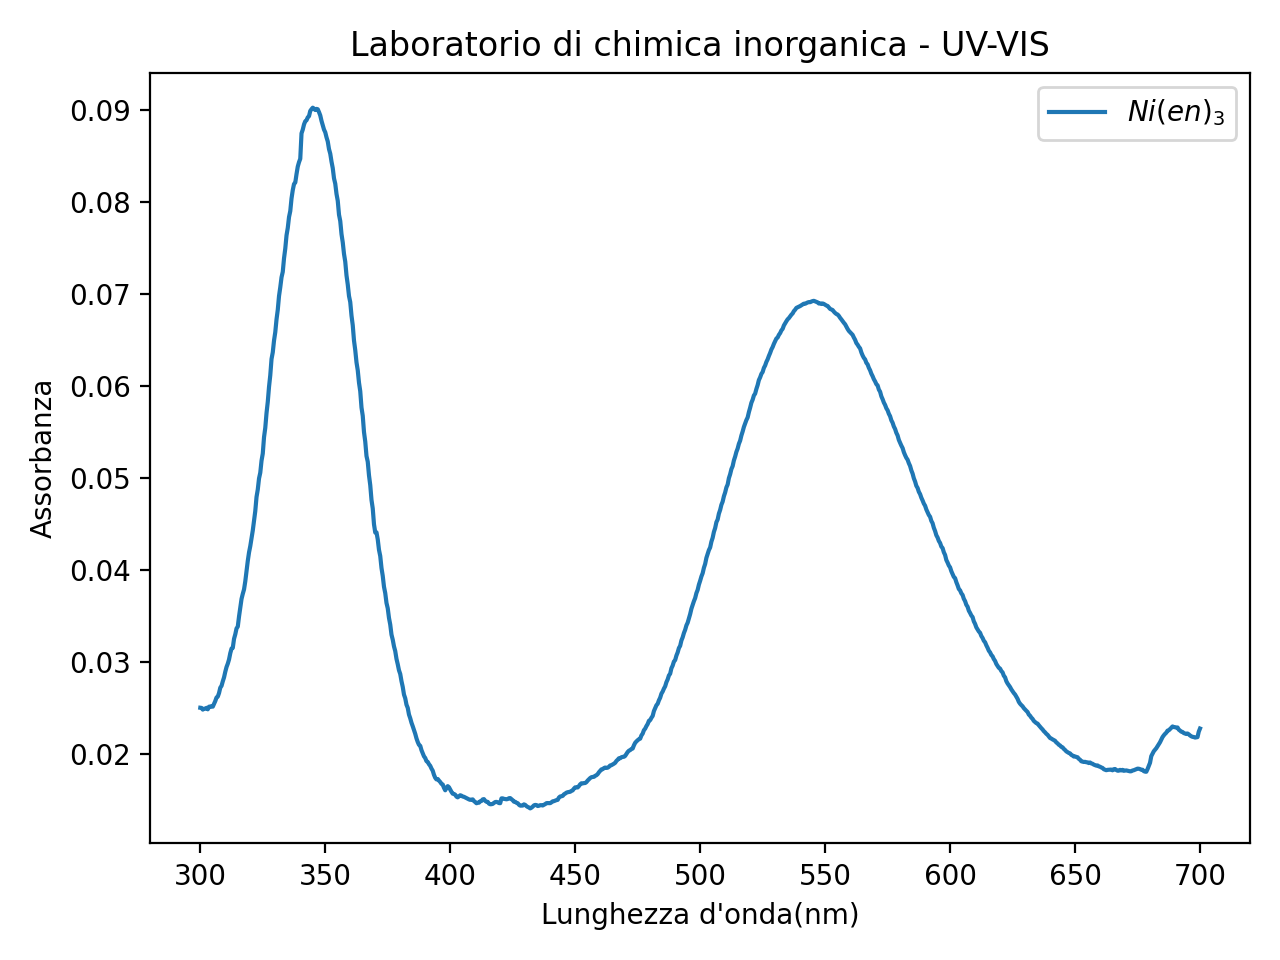
\includegraphics{Relazione/foto/Nienuv.png}
    \caption{Spettro UV-VIS \ce{[Ni(en)3]Cl2}}
    \label{fig:nienuv}
\end{figure}

\subsubsection{Commenti e osservazioni}
Prima di confrontare i tre spettri ricordiamo preliminarmente che il nichel(II) è un centro $d^8$. Pertanto, facendo uso ad esempio dei diagrammi di TanabeSugano, possiamo prevedere che ci siano tre bande di assorbimento relativamente $^1$ intense dovute alle tre transizioni spin-permesse dallo stato fondamentale ${ }^3 A_{2 g}$ verso i tre stati eccitati ${ }^3 T_{2 g},{ }^3 T_{1 g}(F)$ e ${ }^3 T_{1 g}(P)$. Troviamo conferma delle nostre previsioni guardando lo spettro del complesso della trisetilendiammina, mentre per gli altri due vediamo solo due bande. La cosa tuttavia non ci sorprende in quanto sappiamo che l'etilendiammina è il legante a campo più forte fra quelli di cui abbiamo gli spettri e quindi possiamo supporre che negli altri casi la banda ad energia più bassa sia semplicemente uscita dalla finestra di misurazione. Possiamo sfruttare proprio l'informazione spettroscopica per valutare quale sia lo splitting di campo cristallino indotto dalla presenza dei leganti. Se avessimo i massimi della banda a più bassa energia non ci sarebbe nessuna difficoltà in quanto l'energia corrisponderebbe proprio al $\Delta_o$. Purtroppo, non essendo visibile, dobbiamo arrangiarci con le altre due bande e con i diagrammi di Tanabe-Sugano. Ad esempio, per $\mathrm{Ni}\left(\mathrm{NH}_3\right)_6 \mathrm{Cl}_2$ possiamo calcolare il rapporto fra le energie delle due transizioni
$$
\frac{E_3 A_{2 g} \rightarrow{ }^3 T_{1 g}(P)}{E_3 A_{2 g} \rightarrow{ }^3 T_{1 g}(F)}=\frac{\lambda_F}{\lambda_P}=\frac{545 \mathrm{~nm}}{345 \mathrm{~nm}}=1.58
$$
Adesso, cercando sul diagramma di Tanabe-Sugano per un centro $d^8$ il valore di $\Delta_o / B$ per cui c'è questo stesso rapporto fra le ordinate degli stati coinvolti ricaviamo $\Delta_o / B=14.98$. Leggiamo inoltre dal grafico che la differenza in energia fra le due bande vale $13.40 \mathrm{E} / \mathrm{B}$. Ma poiché questa differenza di energia è nota dallo spettro, possiamo ricavare il valore dello splitting dovuto ai leganti come
$$
\Delta_o=\left[\frac{14.98}{13.40} \cdot\left(\frac{1}{345 \mathrm{~nm}}-\frac{1}{545 \mathrm{~nm}}\right)\right]^{-1}=841 \mathrm{~nm}
$$
Il risultato sembra ragionevole in quanto dalla porzione di banda che si vede nello spettro si può indovinare la presenza di un massimo proprio intorno a questa lunghezza d'onda. Ripetendo lo stesso procedimento per $\mathrm{Ni}\left(\mathrm{NH}_3\right)_6 \mathrm{Cl}_2$ si ottiene $\Delta_o=893 \mathrm{~nm}$ che corrisponde, come atteso, ad un'energia minore rispetto al caso precedente. Il complesso di esaacquonichel è più complicato poiché presenta una banda sdoppiata dovuta, a quanto ho visto in letteratura, al fatto che i livelli ${ }^3 T_{1 g}(F)$ e ${ }^1 E_g$ siano quasi degeneri per il valore di splitting indotto dall'acqua e che quindi possano accoppiare fra loro. Non è quindi semplice decidere quale frequenza prendere, ma si possono ottenere valori di $\Delta_o$ compresi fra $800 \mathrm{~nm}$ e $1050 \mathrm{~nm}$.



\subsection{Caratterizzazione tramite misura magnetica}
Abbiamo eseguito 4 misure per ciascun composto alla bilancia Johnson Matthey. La costante della bilancia valeva $C = 1.087 \cdot 10^{-9}$ e la temperatura risultava di 24 °C.
I dati raccolti si possono trovare in \autoref{sec:dati} nella \autoref{tab:magnet}



\begin{table}[ht!]
\centering
\textbf{Risultati}

\begin{tabular}{lcc}
 \hline 
 Composto & $\chi (10^{-6})$[$\mathrm{cm^3/g}$]  & Incertezza    \\
\hline\hline 
 \multirow{4}{*}{$\left[\mathrm{Ni}\left(\mathrm{Et}_2 \mathrm{en}\right)_2\left(\mathrm{H}_2 \mathrm{O}\right)_2\right] \mathrm{Br}_2$} & 8.337 & .410 \\ 

& 8.191 & .355 \\
& 8.148 & .434 \\
&8.245& .403  \\
\hline
Media & 8.230 & \\
$\sigma$ & .057 & \\
\hline
 \multirow{4}{*}{ \ce{[Ni(en)3]Cl2}} & 9.625 & .513  \\ 
 & 9.675 & .454  \\
& 9.744 & .436  \\
& 9.624 & .514  \\ \hline
Media & 9.668 & \\
$\sigma$ & .056 & \\


 
\hline
\end{tabular}

\caption{Misure della suscettibilità magnetica con relativa incertezza. Deviazione standard e media delle misure}
\label{tab:magn}
\end{table}


Calcoliamo la suscettibilità magnetica molare tramite la seguente formula:

\[ \chi_m =  \chi_s M \]


\begin{table}[ht!]
\centering
\begin{tabular}{lcc}
 &\ce{[Ni(en)3]Cl2}    &  \ce{[Ni(Eten)2(H2O)2]Br2} \\ \hline
 [$\mathrm{cm^3/mol} \cdot $] $10^{-3}$ &  2.85  & 4.72\\
\end{tabular}
\end{table}

\[ \chi'_m = \chi_m - \chi_{\ce{dia}}\]
\[\chi_{\ce{dia}} = \sum_i \nu_i \chi_{\ce{pascal}}\]
\[ \frac{\mu}{\mu_B} = 2.828\sqrt{\chi'_m T}\]
\[ \frac{\mu}{\mu_B} = \sqrt{n(n+1)}\]

\begin{table}[ht!]
\centering
\begin{tabular}{l ccccc r}\hline
& \ce{en} & \ce{Cl} & \ce{H2O} & \ce{Eten} & \ce{Br} & Contributo totale \\
\hline\hline
Correzione diamagnetica & 0.046 & -0.0234 & -0.013 & -0.073 & -0.0346 &  \\
$\nu_i$ \ce{[Ni(en)3]Cl2}  & 3 & 2 & 2 & 0 & 0&-0.2108 \\
 $\nu_i$ \ce{[Ni(Eten)2(H2O)2]Br2}& 0 & 0 & 2 & 2 & 2 & -0.2412\\\hline
\end{tabular}
\end{table}

\begin{table}[ht!]
\centering
\begin{tabular}{ccccc}
Composto& Temperatura[°C] & $\chi'_m$ & $\mu$[$\mu_B$] & n \\
\hline
\ce{[Ni(en)3]Cl2} & 24 & 0.214 & 6.40 & 2.08 \\
\ce{[Ni(Eten)2(H2O)2]Br2} & 24 & 0.246 & 6.87 & 2.17 \\
\end{tabular}
\end{table}

Calcolo 